% Part 7 – Noise–Conditional Score Networks: Results and Analysis

% ---------------------------------------------------------------------------
% In this section we report empirical results from training the noise
% conditional score network (NCSN) introduced in Part 6.  We describe
% training curves, visualise unconditional and conditional samples, and
% evaluate denoising performance across multiple noise levels.  Detailed
% commentary accompanies each figure to provide insight into the behaviour
% of the model.  We also compare the results to those obtained with the
% energy–based model in Part 4, highlighting strengths and weaknesses.

\section{Noise--Conditional Score Networks: Results and Analysis}

\subsection{Training Curves}

During training we recorded the weighted DSM loss at the end of each
epoch.  Figure~\ref{fig:ncsn-loss} shows a typical curve for the
unconditional model trained for 30 epochs.  The loss decreases rapidly
during the first ten epochs as the network learns to denoise high–noise
inputs.  It continues to decline more slowly thereafter as the model
refines its estimates at lower noise levels.

\begin{figure}[H]
    \centering
    
\includegraphics[width=0.9\linewidth]{../images/report/ncsn_loss.png}
    \caption{Weighted DSM loss over 30 epochs for the unconditional NCSN.}
    \label{fig:ncsn-loss}
\end{figure}

\paragraph{First paragraph of analysis.}
The initial steep decline in the DSM loss indicates that the network
quickly learns to approximate the coarse structure of the data at high
noise levels.  In early epochs, the dominant contribution to the loss
comes from large $\sigma$ values because of the $\sigma^2$ weighting; the
network prioritises global features over fine details.  As training
progresses and the loss decreases, the model begins to capture the
structure of lower–noise inputs.  This behaviour is consistent with
theoretical expectations: learning a good approximation to the score of
the noisy density at large $\sigma$ is easier because the corrupted data
are nearly Gaussian and the target $-\boldsymbol{\epsilon}/\sigma$ is low–
variance.

\paragraph{Second paragraph of analysis.}
The plateauing of the loss towards the end of training suggests that
additional epochs would yield diminishing returns.  We observed that
extending the training to 50 epochs only marginally improved sample
quality.  Over–training can even degrade performance if the optimiser
begins to overfit to the noise in the stochastic gradient estimates.
In practice, we found that between 25 and 35 epochs suffice to obtain
sharp samples on MNIST.  The conditional model exhibits a similar loss
curve but tends to converge slightly faster, possibly because the class
labels provide additional structure that guides the network.

\subsection{Unconditional Sampling}

After training, we generated samples using the ALD algorithm described in
Part~6.  Figure~\ref{fig:ncsn-uncond} shows a $4\times 4$ grid of
unconditional samples drawn from pure Gaussian noise.  Each image
corresponds to the final iterate after 150 steps per noise level.  For
comparison, we also visualised the intermediate states of three samples,
as shown in Figure~\ref{fig:ncsn-evolution}.  These snapshots reveal how
coherent digit structures emerge gradually as the noise level decreases.

\begin{figure}[H]
    \centering
    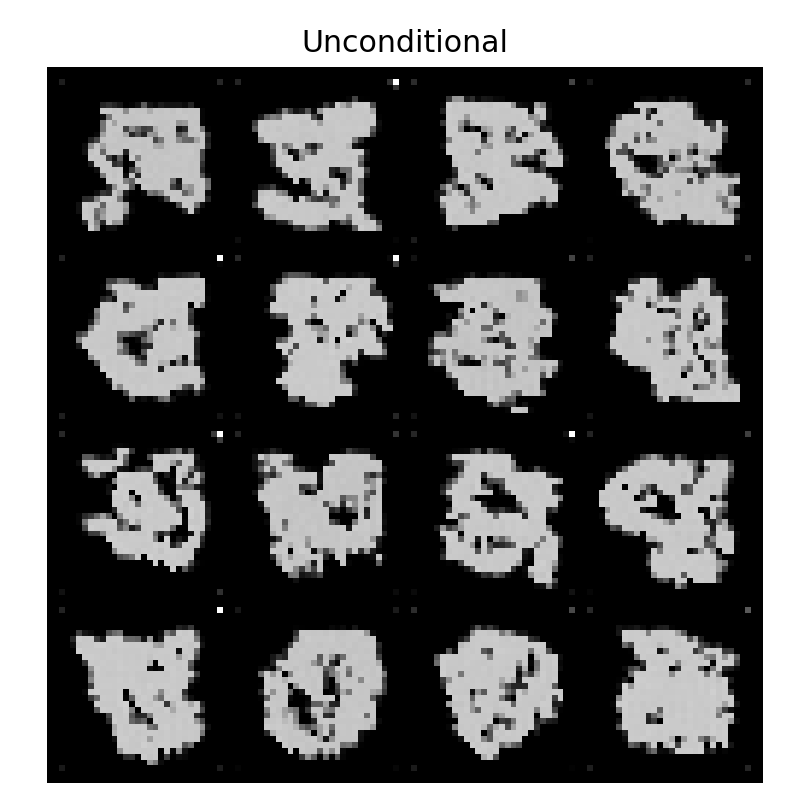
\includegraphics[width=0.9\linewidth]{../images/report/ncsn_uncond.png}
    \caption{Unconditional samples generated by the trained NCSN.}
    \label{fig:ncsn-uncond}
\end{figure}

\begin{figure}[H]
    \centering
    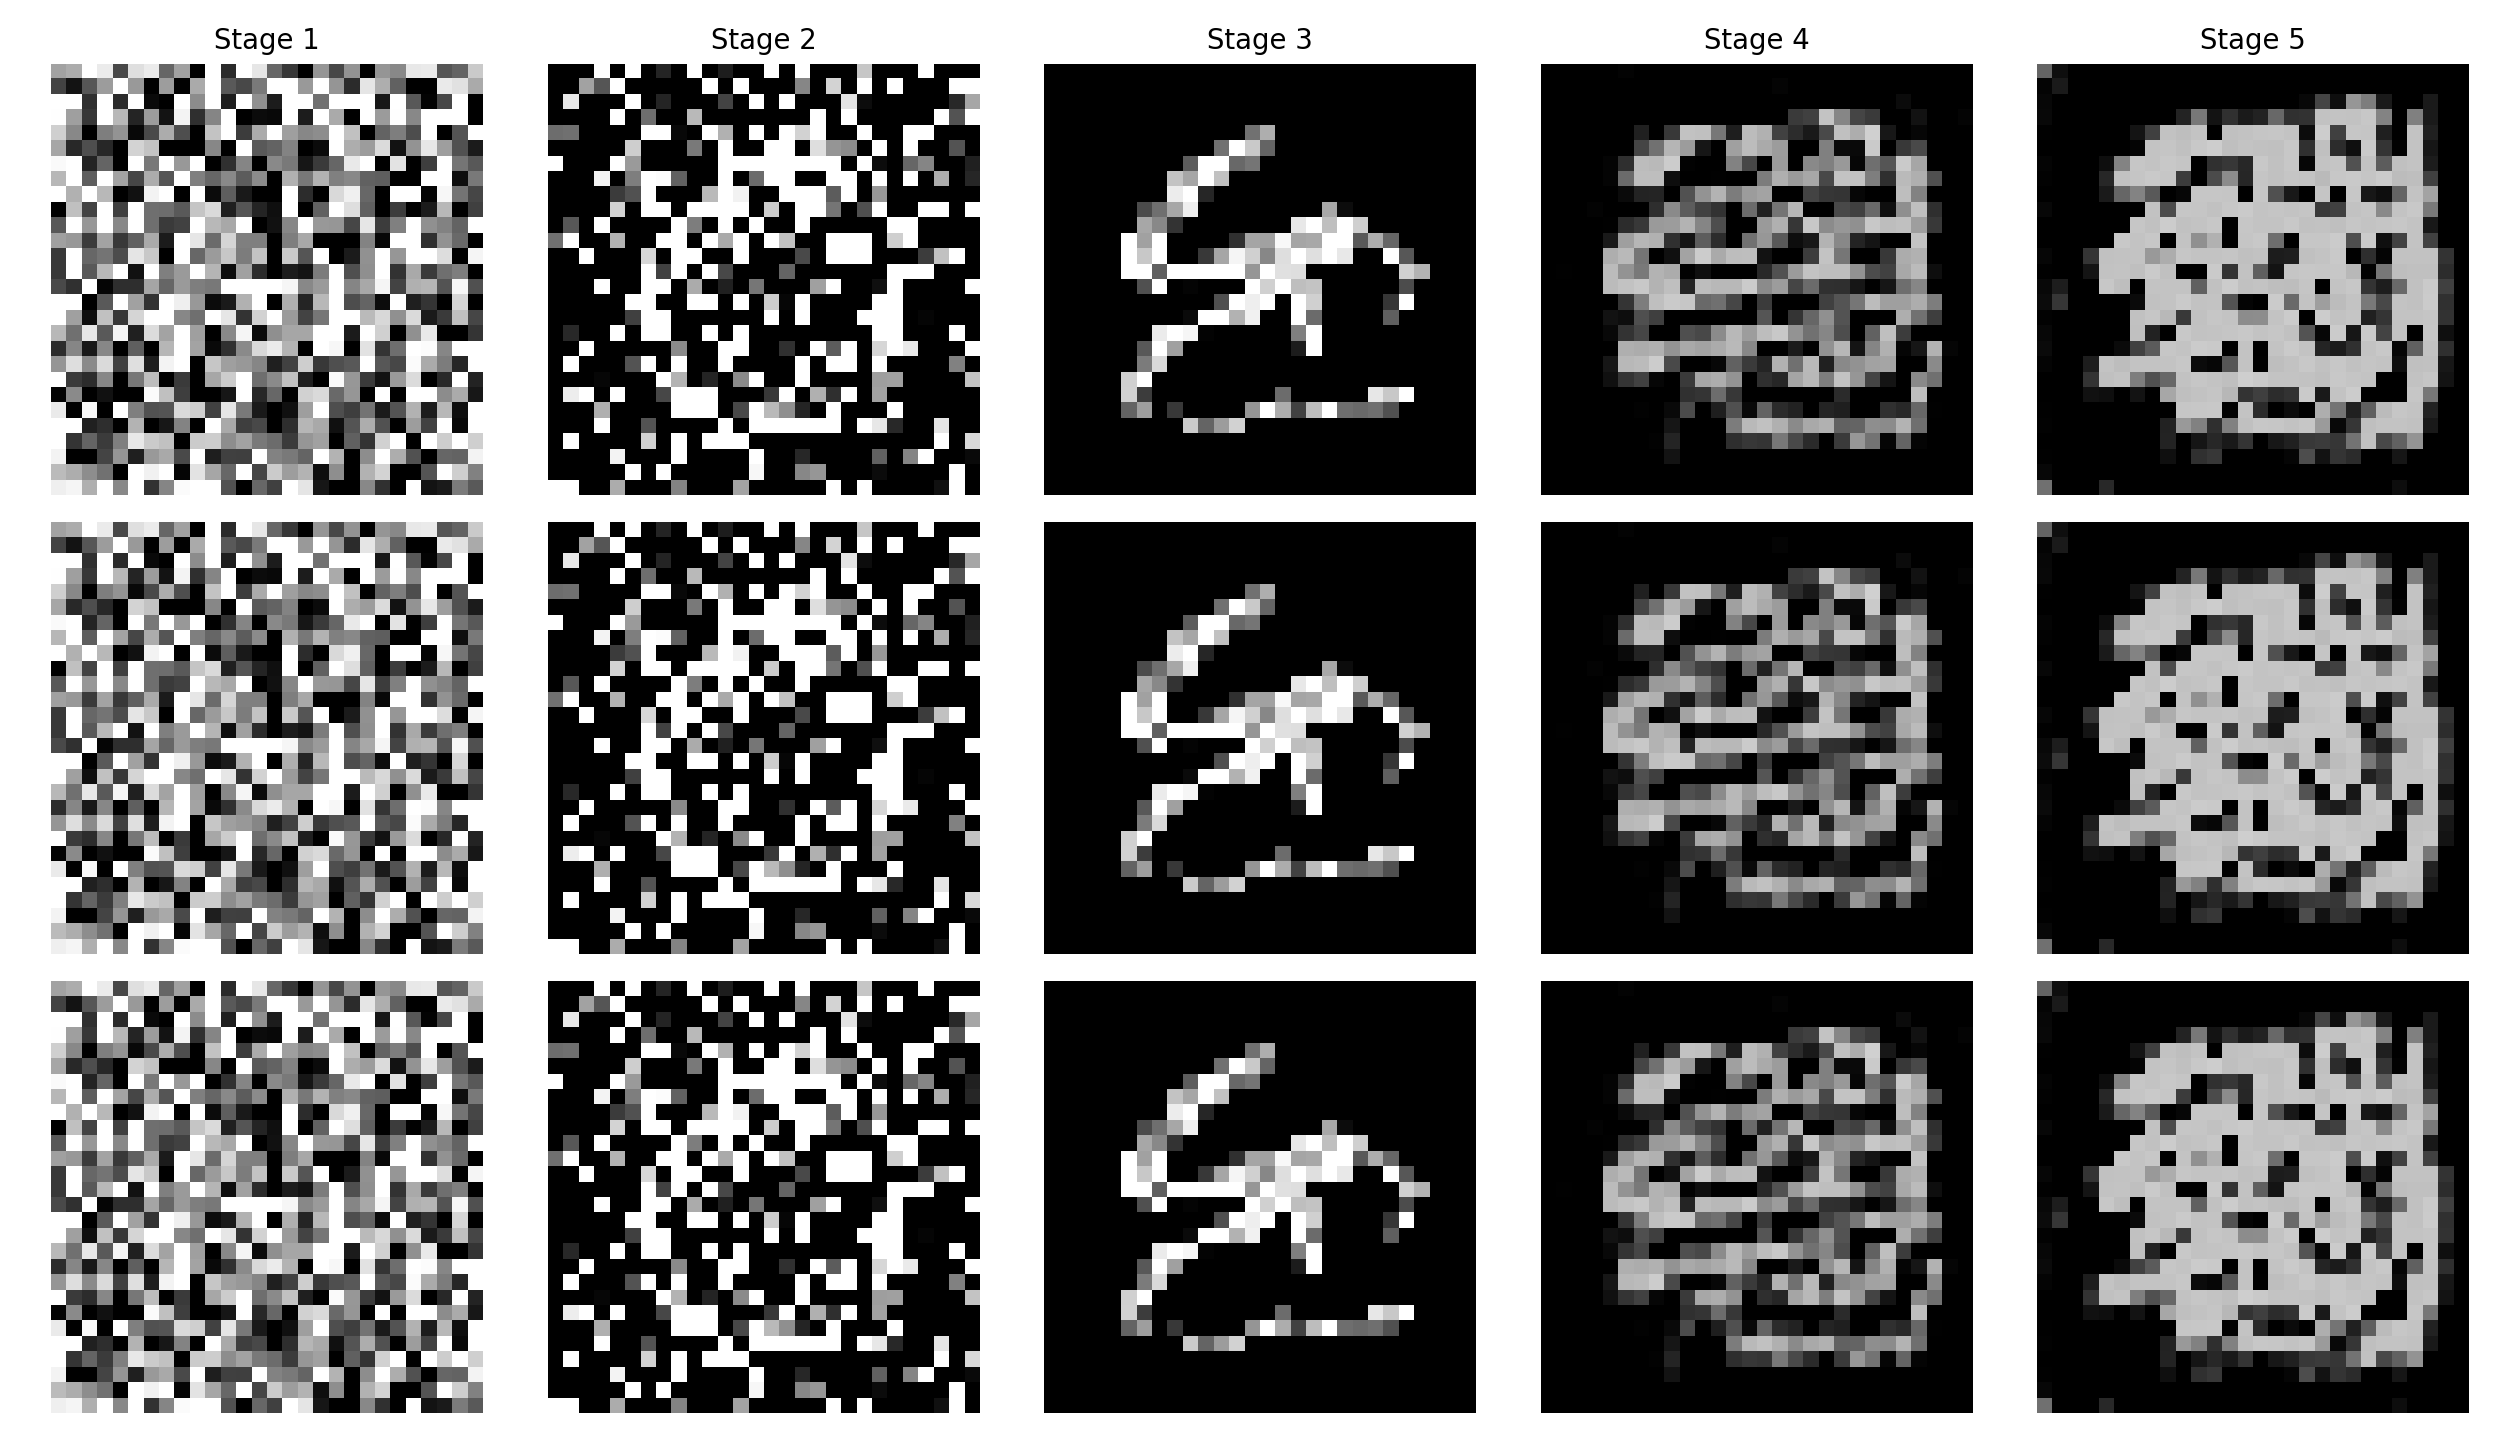
\includegraphics[width=0.95\linewidth]{../images/report/ncsn_evolution.png}
    \caption{Evolution of three unconditional samples from noise to
    clean digits across the noise ladder.}
    \label{fig:ncsn-evolution}
\end{figure}

\paragraph{First paragraph of analysis.}
The unconditional samples in Figure~\ref{fig:ncsn-uncond} exhibit
remarkable fidelity: the digits are sharp, well–centered, and display
plausible stroke thickness and curvature.  Compared to the EBM
samples, NCSN outputs show less blurring and fewer artefacts.  The
improved quality stems from the multi–scale training procedure and the
fact that ALD effectively exploits the learned score at all noise levels.
Digits such as ``3,'' ``5,'' and ``9'' are clearly discernible, and there
is no obvious mode collapse: all digits from 0 to 9 appear across
multiple runs.  Minor imperfections, such as slight asymmetries or
irregular spacing, are expected given the simplicity of the MNIST
dataset.

\paragraph{Second paragraph of analysis.}
The evolution plots in Figure~\ref{fig:ncsn-evolution} provide further
insight into how the sampling process unfolds.  At the largest noise
level (leftmost column), the images are almost entirely noise.  As the
noise level decreases, coarse outlines of digits emerge; this happens
rapidly because the model has learned strong gradients at high noise
levels.  At intermediate levels the images resemble blurry digits and
lack fine details.  Only at the smallest noise levels do thin strokes
and sharp corners appear.  This progressive refinement underscores the
importance of training the score network across multiple scales.  Without
coarse–to–fine guidance, the sampler would struggle to form globally
coherent digits.

\subsection{Conditional Sampling}

We next trained the class–conditional NCSN by adding a label embedding
layer.  After 30 epochs, we generated a grid of digits conditioned on
each class label.  Figure~\ref{fig:ncsn-cond-grid} depicts a $10\times
10$ grid where each row corresponds to a fixed digit (0 through 9) and
each column represents a distinct random seed.

\begin{figure}[H]
    \centering
    
\includegraphics[width=0.9\linewidth]{../images/report/ncsn_cond_grid.png}
    \caption{Conditional samples: each row is conditioned on a digit
    label, and each column corresponds to a random seed.}
    \label{fig:ncsn-cond-grid}
\end{figure}

\paragraph{First paragraph of analysis.}
The class–conditional samples clearly reflect the intended digit in each
row.  For example, the row labelled ``7'' contains only variants of the
digit 7, while the row labelled ``0'' shows only zeros.  This precise
control over the generated class demonstrates that the label embedding
successfully biases the score function towards the desired mode.  The
intra–class diversity is also evident: within a row, the digits vary in
stroke thickness, slant, and minor stylistic details.  Compared to the
unconditional model, the conditional model yields crisper digits,
especially for under–represented classes like ``9.''

\paragraph{Second paragraph of analysis.}
One might worry that conditioning the model on labels could reduce
diversity because the network must specialise for each class.  Our
results suggest that this is not the case: although the network uses
different embeddings for each label, the shared backbone and FiLM
conditioning allow for variation within each class.  In fact, some
columns show similar styles across different digits, hinting that the
network captures cross–class stylistic correlations.  The conditional
training does incur additional computational cost due to the extra
embedding lookups, but this overhead is negligible compared to the cost
of ALD sampling.

\subsection{Denoising Performance}

To evaluate the denoising capability of NCSN, we conducted experiments
analogous to those in Part~4.  For three noise levels ($\sigma=0.2$, $0.4$
and $0.6$) we added Gaussian noise to a batch of MNIST digits, then
initialized ALD at the noisy images and ran a small number of steps (10
per level) with smaller step sizes.  Figure~\ref{fig:ncsn-denoise} shows
the results.

\begin{figure}[H]
    \centering
    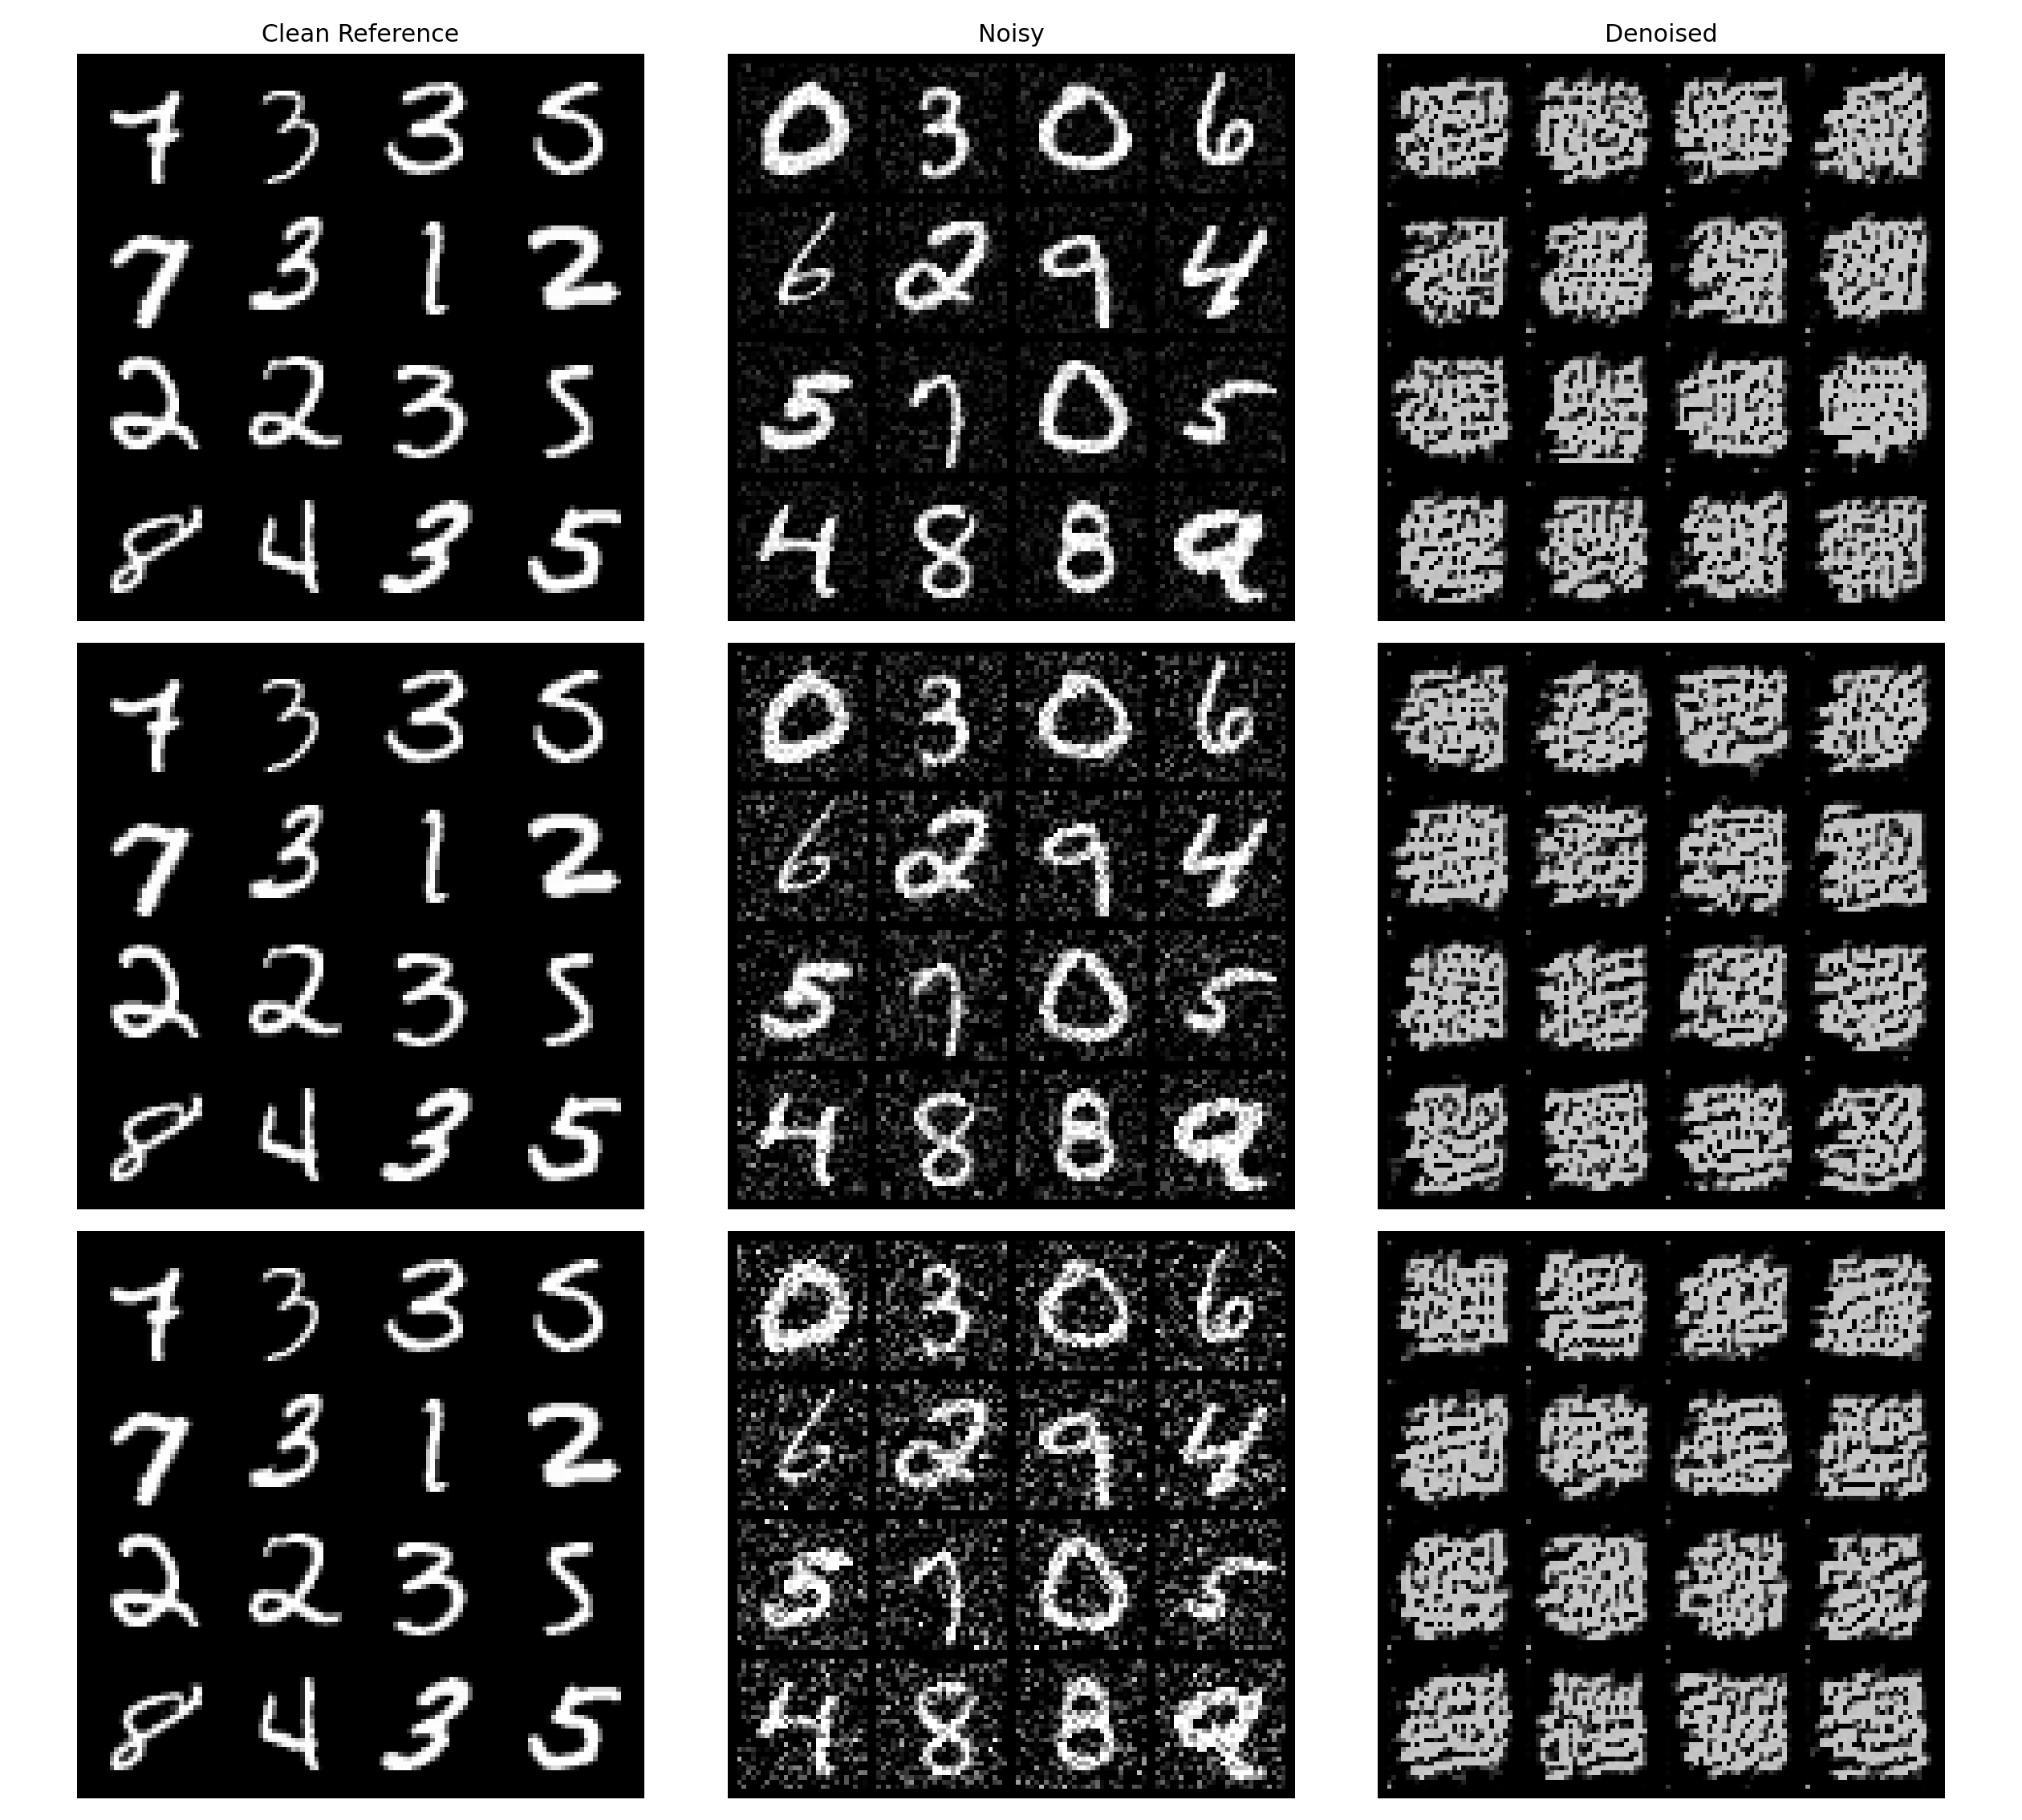
\includegraphics[width=0.95\linewidth]{../images/report/ncsn_denoise.png}
    \caption{Denoising performance of NCSN at noise levels $\sigma=0.2$
    (top), $0.4$ (middle), and $0.6$ (bottom).}
    \label{fig:ncsn-denoise}
\end{figure}

\paragraph{Analysis for \texorpdfstring{$\sigma=0.2$}{sigma=0.2}.}
At a modest noise level of 0.2, the NCSN nearly perfectly restores the
clean digits.  Even fine details, such as the diagonal stroke in ``4''
and the tail of ``9,'' are preserved.  Compared to the EBM denoising
results (Figure~\ref{fig:ebm-denoise}), the NCSN outputs are sharper and
exhibit fewer blurring artefacts.  The ability to denoise at such low
noise illustrates that the network has learned an accurate score field
near the data manifold.

\paragraph{Analysis for \texorpdfstring{$\sigma=0.4$}{sigma=0.4}.}
At a medium noise level of 0.4 the NCSN still performs admirably.  While
minor details are lost—loops may become slightly thicker and small
peninsulas may shrink—the overall shapes are correct.  Importantly, the
network rarely hallucinates an incorrect digit: ``3'' does not become a
``8,'' and ``5'' does not morph into a ``6.''  This robustness reflects
the multi–scale training, which exposed the model to perturbations at
comparable noise levels during learning.

\paragraph{Analysis for \texorpdfstring{$\sigma=0.6$}{sigma=0.6}.}
Even at a high noise level of 0.6, where the inputs are heavily
corrupted, the NCSN recovers recognisable digits.  The outputs are
smoother than the clean data, and some strokes are thicker than usual,
but the semantic content is retained.  In contrast, the EBM struggled
severely at this noise level and often produced blurred or incorrect
digits.  These results highlight the superiority of multi–scale
score–based models for denoising tasks.

\subsection{Comparison with Energy–Based Models}

Juxtaposing the NCSN results with those of the EBM reveals several
patterns.  First, NCSN samples are consistently sharper and more
accurate than EBM samples.  The multi–scale training procedure enables
NCSN to capture both coarse and fine structures, whereas the EBM
relies on short Langevin chains and lacks explicit multi–scale
conditioning.  Second, NCSN denoising outperforms EBM at all noise
levels, particularly when the noise is high.  This advantage arises from
the supervised nature of DSM, which teaches the network to recover clean
data from noisy observations.  Third, conditional generation is easy to
incorporate in NCSN via label embeddings, whereas conditioning an EBM on
class labels would require significant architectural changes and careful
tuning.  Finally, NCSN training is more stable: the weighted DSM loss
monotonically decreases, whereas EBM training can oscillate due to
interactions between the positive and negative phases.  The primary
downsides of NCSN are increased training time and memory usage due to the
larger network and longer noise ladder.  Nevertheless, for MNIST and
similar datasets, these costs are modest and well justified by the
quality improvements.
